\documentclass{standalone}
\usepackage{graphicx}
\usepackage{tikz}
\usepackage{hsbcommon}
\begin{document}
    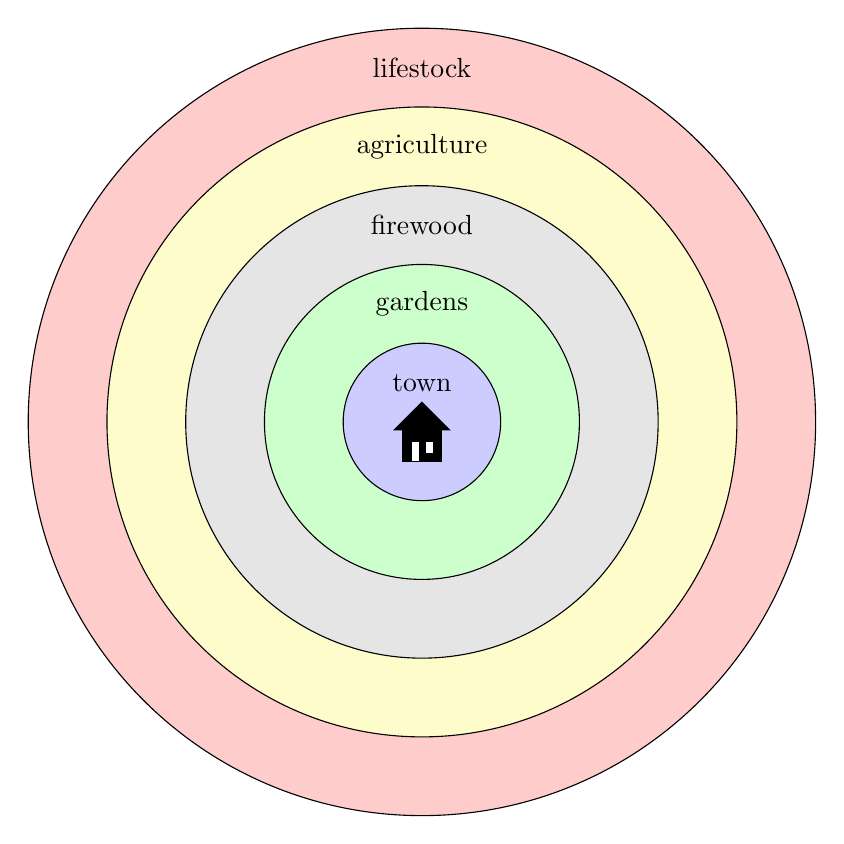
\begin{tikzpicture}
    \tikzset{
        myhome/.pic={
        \filldraw (0,0) rectangle (0.5,0.4);
        \filldraw (-0.1,0.4) -- (0.25,0.75) -- (0.6,0.4) -- cycle;
        \filldraw[white,draw=black] (0.12,0) rectangle (0.22,0.25);
        \filldraw[white,draw=black] (0.3,0.1) rectangle (0.4,0.25);
        }
    }
        \foreach [count=\i] \ii/\mycol in 
        {
            lifestock/red,
            agriculture/yellow,
            firewood/gray,
            gardens/green,
            town/blue%
        }
        {
            \draw[fill=\mycol!20] (0:0) circle (6-\i);
            \node at (90:6-\i-0.5) {\ii};
        }
        \draw (-0.25,-0.5) pic {myhome};
    \end{tikzpicture}
\end{document}